\section{Results}\label{sec:results}

\subsection{The engine across the circuit cases}\label{sec:results-engine}

Figure~\ref{fig:physics} and Table~\ref{tab:cases} give the coupled engine over the circuit. The engine reproduces the size-reduction ladder
of a crushing circuit: the gyratory case G01 gives a coarse product ($P_{80}=153.6$~mm) at a high throughput ($4629$~t/h) with a reduction
ratio of $1.17$; the jaw J01 an intermediate product ($126.4$~mm at $923$~t/h); the secondary cone S01 $27.7$~mm at $643$~t/h and a reduction
ratio of $4.55$; the tertiary cone T01 $7.1$~mm at $240$~t/h; and the short-head cone H01 $4.6$~mm at $216$~t/h, the finest product of the
set. Within the secondary class the setting and the speed move the product as expected: S03, run past the speed optimum at $470$~rpm, gives
$856$~t/h on the falling side of its hump (Figure~\ref{fig:sweeps}(a)), and S06, at a setting of $12$~mm, the finest secondary product
($9.1$~mm) with a reduction ratio of $9.80$, above the typical ceiling of one stage and flagged as such. The setting sweep of S01
(Figure~\ref{fig:sweeps}(b)) shows the trade-off a process engineer reads: between $16$ and $48$~mm, $P_{80}$ rises from about $14$ to $42$~mm and
the throughput from about $420$ to $860$~t/h, both close to linear, because the capacity is linear in the setting at a fixed throw and speed and
the classification window moves with the setting. The three controls behave as stated: CP1 is pass-through with a reduction ratio of $1.12$,
CI1 is invalid with a reduction ratio of one and zero power, and CK1 is a valid choke point. Every case lies inside its declared expected ranges,
otherwise the bake would have stopped. What this shows is that the coupled models behave as the cited models are known to behave; it is not a
validation against a plant, which only the HP500 lane can give.

\begin{figure}[!t]
\centering
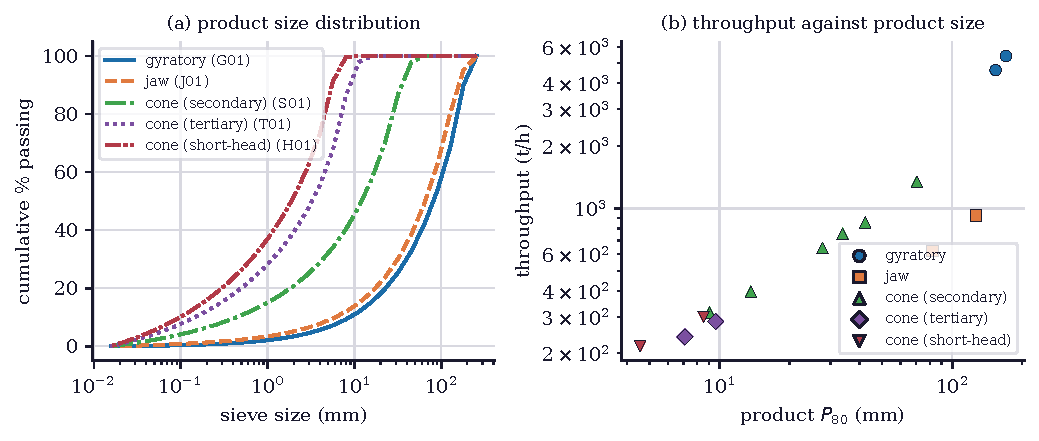
\includegraphics[width=\textwidth]{fig-physics.pdf}
\caption{The coupled engine over the circuit cases, from the committed traces: (a) product size distributions of one gyratory (G01), jaw (J01),
secondary cone (S01), tertiary cone (T01) and short-head cone (H01) case; (b) product $P_{80}$ against throughput for the seventeen circuit cases,
by machine type.}
\label{fig:physics}
\end{figure}

\subsection{Benchmark on the ten HP500 surveys}\label{sec:results-bench}

Table~\ref{tab:bench} gives every predictor on the same ten surveys under strict leave-one-survey-out, and Figure~\ref{fig:loo} the held-out
predictions against the measured values. On throughput the predictors that use the setting and the capacity physics sit between $12.00\%$ and
$13.67\%$, within the noise of ten surveys of each other, and all beat the constant mean ($18.29\%$); the label-shuffle control ($25.04\%$) is
worse than the backbone, as it must be. The calibrated backbone, with one fitted scalar and the engine's shape, matches the two-coefficient
free-form fit ($12.09\%$ against $12.18\%$), and its in-sample error is $11.55\%$, so its held-out number is not an artifact of the fit. The
bounded residual does not improve on the backbone held out ($13.45\%$), the null result stated as the expectation before the run.

On power the picture is different. The calibrated backbone, whose power is the Bond draw refit in the published form, is worse than the constant
mean ($25.94\%$ against $24.48\%$, held-out $R^2=-0.62$), because the Bond draw is nearly flat while the measured power is not
(Section~\ref{sec:m-bond}). The setting-only line is the best power predictor ($12.78\%$, $R^2=0.48$), followed by the free-form fit
($14.03\%$), CrusherBayes ($14.31\%$) and Morrell with a no-load term ($15.21\%$). CrusherBayes is $1.53$ points behind the line, within the noise
of $n=10$ and not a gain; Morrell through the origin, at $38.08\%$, is the worst size-aware model. The mean log predictive densities
(Table~\ref{tab:lpd}) rank the four predictive distributions the same way: on power the line ($-5.341$) and CrusherBayes ($-5.346$) are tied and
the backbone band is the worst ($-5.847$); on throughput the free-form fit ($-6.647$) and CrusherBayes ($-6.678$) are ahead of the line
($-6.709$) and the backbone ($-6.896$), by differences that one survey can reverse.

\begin{table}[!t]
\centering
\caption{Strict leave-one-survey-out scores of every predictor on the same ten HP500 surveys: MAPE in percent, RMSE in the unit of the target,
held-out $R^2$, coverage of the $80\%$ interval and its mean width in the unit of the target. Residual-band predictors carry the nested band of
their own held-out residuals; CrusherBayes carries its posterior predictive interval. A dash marks a score that is not defined. Generated from
\texttt{loo.json} and \texttt{crusherbayes.json}.}
\label{tab:bench}
\scriptsize
% generated by figures/make_tables.py; do not edit by hand
\begin{tabular}{@{}l rrrrr rrrrr@{}}
\toprule
 & \multicolumn{5}{c}{Throughput (t/h)} & \multicolumn{5}{c}{Power (kW)} \\ \cmidrule(lr){2-6}\cmidrule(lr){7-11}
Method & MAPE & RMSE & $R^2$ & Cov. & Width & MAPE & RMSE & $R^2$ & Cov. & Width \\
\midrule
Constant mean & $18.29$ & $258.5$ & $-0.235$ & -- & -- & $24.48$ & $68.5$ & $-0.235$ & -- & -- \\
Label-shuffle control & $25.04$ & $322.8$ & $-0.925$ & -- & -- & $40.19$ & $110.5$ & $-2.214$ & -- & -- \\
Calibrated backbone & $12.09$ & $176.7$ & $0.423$ & $0.80$ & $473.8$ & $25.94$ & $78.5$ & $-0.622$ & $0.90$ & $209.8$ \\
Backbone with bounded residual & $13.45$ & $189.5$ & $0.337$ & -- & -- & $25.37$ & $92.1$ & $-1.231$ & -- & -- \\
Free-form fit on CSS and $f_{80}$ & $12.18$ & $174.4$ & $0.438$ & $0.80$ & $468.5$ & $14.03$ & $48.7$ & $0.377$ & $0.80$ & $129.8$ \\
Setting-only line & $13.67$ & $177.8$ & $0.416$ & $0.80$ & $478.8$ & $12.78$ & $44.6$ & $0.478$ & $0.80$ & $119.6$ \\
Morrell, through the origin & -- & -- & -- & -- & -- & $38.08$ & $111.7$ & $-2.281$ & -- & -- \\
Morrell with a no-load term & -- & -- & -- & -- & -- & $15.21$ & $46.5$ & $0.430$ & -- & -- \\
CrusherBayes (posterior predictive) & $12.00$ & $168.6$ & -- & $0.80$ & $439.1$ & $14.31$ & $44.7$ & -- & $0.90$ & $117.7$ \\
\bottomrule
\end{tabular}

\end{table}

\begin{figure}[!t]
\centering
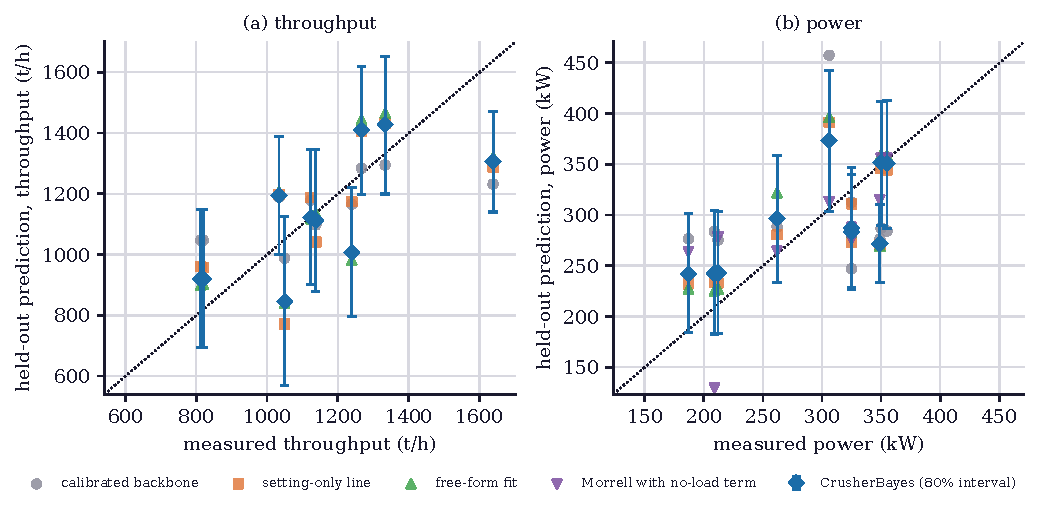
\includegraphics[width=\textwidth]{fig-loo.pdf}
\caption{Held-out predictions against the measured values on the ten HP500 surveys, for (a) throughput and (b) power: the calibrated backbone, the
free-form fit, the setting-only line and, for power, Morrell with a no-load term, and the CrusherBayes predictive mean with its $80\%$ interval. The
dotted line is parity.}
\label{fig:loo}
\end{figure}

\begin{table}[!t]
\centering
\caption{Mean log predictive density of the held-out surveys for the four predictors that give a distribution: three residual-band predictors with
their nested Gaussian band and CrusherBayes with its posterior predictive. Higher is better. Generated from \texttt{crusherbayes.json}.}
\label{tab:lpd}
\footnotesize
% generated by figures/make_tables.py; do not edit by hand
\begin{tabular}{@{}l rr@{}}
\toprule
Method & Throughput & Power \\
\midrule
Setting-only line & $-6.709$ & $-5.341$ \\
Calibrated backbone & $-6.896$ & $-5.847$ \\
Free-form fit & $-6.647$ & $-5.399$ \\
CrusherBayes & $-6.678$ & $-5.346$ \\
\bottomrule
\end{tabular}

\end{table}

\subsection{Optimism of an evaluation that leaks}\label{sec:results-leaky}

Table~\ref{tab:leaky} gives the same predictors when the held-out survey is allowed into its own fit. The fits that adapt most to the data gain
most: the bounded residual falls from $13.45\%$ to $8.51\%$ on throughput and from $25.37\%$ to $12.00\%$ on power, a gap of $13.37$ points, and the
free-form fit from $14.03\%$ to $9.46\%$ on power. The calibrated backbone, with one scalar for throughput, gains $1.14$ points. The label-shuffle
control on power falls from $40.19\%$ to $15.50\%$, a gap of $24.69$ points: a fit of permuted labels looks almost as good as the line when the
survey is in the fit, which is how much of the apparent skill of a leaky evaluation is the fit absorbing the survey. The setting-only line has one
of the smallest gaps ($2.75$ points on power), as a two-coefficient fit on one feature should. An evaluation of a calibrated crusher model on the
surveys it was fitted to would therefore have ranked the bounded residual first on both targets; held out it ranks behind the backbone on
throughput and ties the backbone on power.

\begin{table}[!t]
\centering
\caption{MAPE in percent of every predictor with the held-out survey outside its fit (strict) and inside it (leaky), and their difference in points,
on the same ten surveys and folds. Generated from \texttt{loo.json}.}
\label{tab:leaky}
\footnotesize
% generated by figures/make_tables.py; do not edit by hand
\begin{tabular}{@{}l rrr rrr@{}}
\toprule
 & \multicolumn{3}{c}{Throughput MAPE (\%)} & \multicolumn{3}{c}{Power MAPE (\%)} \\ \cmidrule(lr){2-4}\cmidrule(lr){5-7}
Method & Strict & Leaky & Gap & Strict & Leaky & Gap \\
\midrule
Constant mean & $18.29$ & $16.46$ & $1.83$ & $24.48$ & $22.03$ & $2.45$ \\
Label-shuffle control & $25.04$ & $21.34$ & $3.70$ & $40.19$ & $28.49$ & $11.70$ \\
Calibrated backbone & $12.09$ & $10.95$ & $1.14$ & $25.94$ & $19.28$ & $6.66$ \\
Backbone with bounded residual & $13.45$ & $8.51$ & $4.94$ & $25.37$ & $12.00$ & $13.37$ \\
Free-form fit on CSS and $f_{80}$ & $12.18$ & $8.24$ & $3.94$ & $14.03$ & $9.46$ & $4.57$ \\
Setting-only line & $13.67$ & $10.60$ & $3.07$ & $12.78$ & $10.03$ & $2.75$ \\
Morrell, through the origin & -- & -- & -- & $38.08$ & $33.81$ & $4.27$ \\
Morrell with a no-load term & -- & -- & -- & $15.21$ & $11.50$ & $3.71$ \\
\bottomrule
\end{tabular}

\end{table}

\subsection{The predictive band of the calibrated backbone}\label{sec:results-band}

Table~\ref{tab:band} and Figure~\ref{fig:bands} give the band survey by survey. With $\sigma$ from all ten held-out residuals, the band's half-width
is $238.5$~t/h ($20.8\%$ of the mean throughput) and $105.1$~kW ($36.5\%$ of the mean power), and its in-sample coverage is $0.90$ on both targets.
Nested, with $\sigma_{-i}$ from the other nine residuals, the coverage is $0.80$ on throughput and $0.90$ on power. Two surveys fall outside the
throughput band: survey 1, whose measured feed rate of $1639$~t/h is the largest of the set and $407$~t/h above the backbone, and survey 6, $235$~t/h
below it; survey 9 lies inside by $3$~t/h. On power one survey falls outside, survey 7 ($151$~kW below the backbone), whose feed $f_{80}$ of $140$~mm is
the coarsest of the set. The in-sample coverage of $0.90$ on throughput flatters the band; the nested $0.80$ is the figure a reader can rely on, and
with ten surveys either moves by $0.1$ per survey. The relative half-width on throughput, $20.81\%$, is the lower bound the studio shows as a band on
the synthetic secondary-cone cases, read at run time from the document: an uncalibrated case cannot be more accurate than the same model family once
calibrated.

\begin{table}[!t]
\centering
\caption{The nested $80\%$ band of the calibrated backbone per held-out survey: the held-out residual (measured minus prediction), the standard
deviation $\sigma_{-i}$ of the other nine residuals, the half-width $1.2816\,\sigma_{-i}$ and whether the survey lies inside. Generated from
\texttt{loo.json}.}
\label{tab:band}
\footnotesize
% generated by figures/make_tables.py; do not edit by hand
\begin{tabular}{@{}r rrrl rrrl@{}}
\toprule
 & \multicolumn{4}{c}{Throughput (t/h)} & \multicolumn{4}{c}{Power (kW)} \\ \cmidrule(lr){2-5}\cmidrule(lr){6-9}
Survey & Residual & $\sigma_{-i}$ & Half-width & Inside & Residual & $\sigma_{-i}$ & Half-width & Inside \\
\midrule
1 & $407.1$ & $123.2$ & $157.9$ & no & $-74.7$ & $83.6$ & $107.2$ & yes \\
2 & $-16.8$ & $197.3$ & $252.9$ & yes & $-63.1$ & $84.7$ & $108.6$ & yes \\
3 & $74.2$ & $195.1$ & $250.0$ & yes & $-26.3$ & $86.8$ & $111.2$ & yes \\
4 & $-155.3$ & $189.4$ & $242.8$ & yes & $72.7$ & $81.2$ & $104.1$ & yes \\
5 & $-55.1$ & $196.6$ & $251.9$ & yes & $77.9$ & $80.4$ & $103.1$ & yes \\
6 & $-234.5$ & $178.2$ & $228.4$ & no & $70.8$ & $81.5$ & $104.4$ & yes \\
7 & $61.6$ & $195.7$ & $250.9$ & yes & $-151.3$ & $69.4$ & $89.0$ & no \\
8 & $40.5$ & $196.6$ & $252.0$ & yes & $12.5$ & $86.5$ & $110.9$ & yes \\
9 & $-226.9$ & $179.5$ & $230.0$ & yes & $62.9$ & $82.5$ & $105.7$ & yes \\
10 & $39.2$ & $196.6$ & $252.0$ & yes & $-89.5$ & $81.9$ & $104.9$ & yes \\
\bottomrule
\end{tabular}

\end{table}

\begin{figure}[!t]
\centering
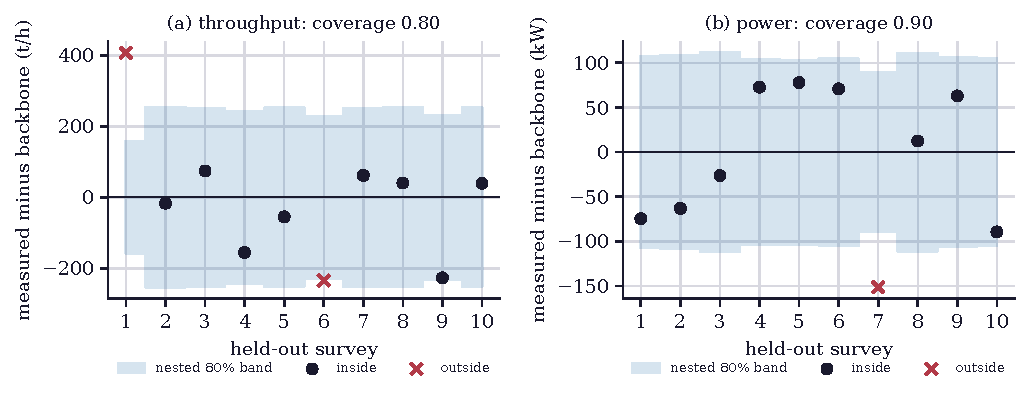
\includegraphics[width=\textwidth]{fig-bands.pdf}
\caption{The held-out residual of the calibrated backbone per survey against its nested $80\%$ band, for (a) throughput and (b) power, with the
surveys outside the band marked by crosses; the nested coverage of each target is in the panel title.}
\label{fig:bands}
\end{figure}

\subsection{Morrell's size-specific energy}\label{sec:results-morrell}

Table~\ref{tab:morrell} and Figure~\ref{fig:morrell} give the two Morrell variants fold by fold. Without a no-load term the fit is one positive
scalar, $M_{ic}$ between $3.70$ and $4.21$~kWh/t across the folds, and the held-out error is $38.08\%$ ($R^2=-2.28$). With a no-load term the error
falls to $15.21\%$, but the fit is not Morrell's physics: in every fold the fitted $M_{ic}$ is negative, from $-6.29$ to $-4.16$~kWh/t, with a no-load
power of $591$ to $727$~kW, about twice the largest measured power of $355$~kW. The measured power falls as the throughput rises (correlation
$-0.85$), and the design column $g_i$ rises with the throughput, so the least-squares line through it has a negative slope and a large intercept. The
variant is a descriptive line on that column and not an estimate of $M_{ic}$ or of a no-load power. Both variants are worse than the setting-only line;
the difference of $2.4$ points for the variant with a no-load term is within the noise, and the $25$ points of the variant without it are not. On these
ten surveys the size-specific energy adds no predictive skill. An SMC Test of the ore and a no-load reading of the machine would replace the two
fitted scalars by measurements and turn the method into a prediction.

\begin{table}[!t]
\centering
\caption{The Morrell fits per fold, each on the nine training surveys: $M_{ic}$ of the variant through the origin, $M_{ic}$ and no-load power of the
variant with a no-load term, and whether that variant's $M_{ic}$ is positive. Generated from \texttt{loo.json}.}
\label{tab:morrell}
\footnotesize
% generated by figures/make_tables.py; do not edit by hand
\begin{tabular}{@{}r rrrl@{}}
\toprule
Held-out survey & $M_{ic}$, origin (kWh/t) & $M_{ic}$, no-load (kWh/t) & $P_{noload}$ (kW) & $M_{ic}>0$ (no-load) \\
\midrule
1 & $4.213$ & $-6.295$ & $726.7$ & no \\
2 & $3.986$ & $-4.458$ & $611.0$ & no \\
3 & $3.915$ & $-4.653$ & $618.4$ & no \\
4 & $3.726$ & $-4.465$ & $601.4$ & no \\
5 & $3.792$ & $-4.727$ & $618.5$ & no \\
6 & $3.703$ & $-4.680$ & $620.2$ & no \\
7 & $3.790$ & $-4.697$ & $622.0$ & no \\
8 & $3.781$ & $-4.639$ & $613.5$ & no \\
9 & $3.709$ & $-4.743$ & $625.2$ & no \\
10 & $4.065$ & $-4.158$ & $590.7$ & no \\
\bottomrule
\end{tabular}

\end{table}

\begin{figure}[!t]
\centering
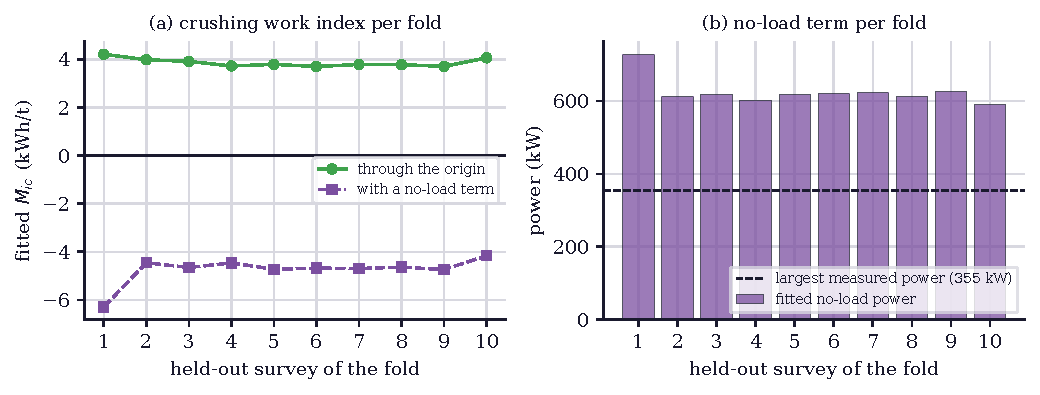
\includegraphics[width=\textwidth]{fig-morrell.pdf}
\caption{The two Morrell variants fold by fold: (a) the fitted crushing work index $M_{ic}$ through the origin and with a no-load term; (b) the fitted
no-load power against the largest measured motor power of the ten surveys.}
\label{fig:morrell}
\end{figure}

\subsection{CrusherBayes: held-out scores, adoption and what the surveys identify}\label{sec:results-cb}

On throughput CrusherBayes has the lowest held-out MAPE ($12.00\%$, RMSE $168.6$~t/h) and the narrowest interval ($439.1$~t/h against $473.8$~t/h for
the backbone band, $7\%$ narrower) at coverage $0.80$; on power its MAPE is $14.31\%$, its interval $117.7$~kW wide, $44\%$ narrower than the backbone
band ($209.8$~kW) at the same coverage of $0.90$, and about the width of the line's band ($119.6$~kW at coverage $0.80$). Table~\ref{tab:adoption}
evaluates the adoption rule term by term. Condition (a) holds: the power MAPE is $1.53$ points above the line's, not three below, and the throughput
MAPE only $0.09$ points below the backbone's. Condition (b) does not hold: both coverages, $0.80$ and $0.90$, lie inside $0.7$ to $0.9$, and both intervals
are narrower than the backbone's band. The rule drops the method only when both conditions hold, so it keeps CrusherBayes. That is the outcome of the
rule as written and not a claim of skill over the line: the method gives a calibrated and narrower interval, and does not predict the power better than
one feature.

\begin{table}[!t]
\centering
\caption{The adoption rule of CrusherBayes evaluated term by term on the held-out scores: the value of CrusherBayes, the reference predictor's value, the
difference, the condition stated before the run and whether CrusherBayes meets it. Generated from \texttt{crusherbayes.json}.}
\label{tab:adoption}
\footnotesize
% generated by figures/make_tables.py; do not edit by hand
\begin{tabular}{@{}l rrr l l@{}}
\toprule
Term of the adoption rule & CrusherBayes & Reference & Difference & Condition & Met \\
\midrule
Power MAPE against the setting-only line (points) & $14.31$ & $12.78$ & $-1.53$ & gain $\geq 3$ & no \\
Throughput MAPE against the backbone (points) & $12.00$ & $12.09$ & $0.09$ & gain $\geq 3$ & no \\
Throughput coverage of the 80\% interval & $0.80$ & -- & -- & $0.7$ to $0.9$ & yes \\
Power coverage of the 80\% interval & $0.90$ & -- & -- & $0.7$ to $0.9$ & yes \\
Throughput mean width (t/h) against the backbone band & $439.1$ & $473.8$ & $34.6$ & not wider & yes \\
Power mean width (kW) against the backbone band & $117.7$ & $209.8$ & $92.0$ & not wider & yes \\
\bottomrule
\end{tabular}

\end{table}

Figure~\ref{fig:contraction} and Table~\ref{tab:contraction} give the contraction of the posterior fitted to all ten surveys. The capacity base is
identified (contraction $0.454$, posterior mean $646.3$~t/h against the nominal $647$), and so are the two noise scales ($0.301$ and $0.332$) and the four
discrepancy slopes on the setting and on $f_{80}$ ($0.340$ to $0.381$). The posterior noise is $145.2$~t/h and $38.8$~kW, much larger than the prior
medians of $60$~t/h and $15$~kW. The discrepancy slope on the setting is large on both targets, $+100.8$~t/h and $-57.1$~kW per standard deviation of the
setting: the engine's dependence on the setting differs from the measured one, on power by about $57$~kW per standard deviation, of the same order as the
slope of the setting-only line ($-8.49$~kW/mm) times the standard deviation of the setting over the ten surveys ($5.94$~mm), about $-50$~kW. The work index, $\zeta$ and $P_n$ contract weakly ($0.854$, $0.733$ and $0.795$), and $\zeta$
and $W_i$ enter the power only as a product. The two classification multipliers, $K_3$, the $t_{10}$ shift and the two discrepancy constants stay at their
prior ($0.878$ to $1.026$). The scalars that set the product size are not identified because the two measured targets carry the product size only through
the Bond term of the power, and the power follows the setting, not the product size. Ten surveys without a measured product size cannot calibrate the
population balance.

\begin{figure}[!t]
\centering
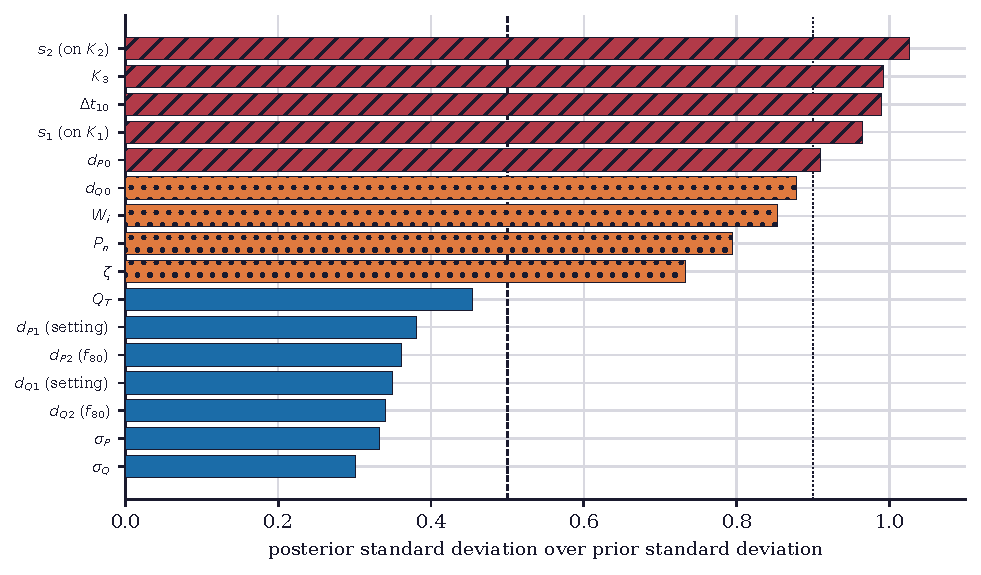
\includegraphics[width=0.85\textwidth]{fig-contraction.pdf}
\caption{Posterior over prior standard deviation of each CrusherBayes parameter for the posterior fitted to all ten surveys. Below $0.5$ (dashed) the surveys
identify the parameter; near one (dotted) it stays at its prior. Plain bars are identified, dotted bars weakly identified, hatched bars not identified.}
\label{fig:contraction}
\end{figure}

\begin{table}[!t]
\centering
\caption{Prior and posterior of every CrusherBayes parameter for the fit to all ten surveys, on the natural scale: prior centre and standard deviation,
posterior mean and standard deviation, and their ratio (the contraction). Discrepancy rows are the exact conditional given the engine scalars. Generated from
\texttt{crusherbayes.json}.}
\label{tab:contraction}
\footnotesize
% generated by figures/make_tables.py; do not edit by hand
\begin{tabular}{@{}l l rrrrr@{}}
\toprule
Parameter & Unit & Prior centre & Prior sd & Posterior mean & Posterior sd & Contraction \\
\midrule
$Q_T$, capacity base & t/h & $647.00$ & $167.01$ & $646.35$ & $75.74$ & $0.454$ \\
$W_i$, blend work index & kWh/t & $9.00$ & $1.52$ & $8.39$ & $1.29$ & $0.854$ \\
$\zeta$, power slope & -- & $1.30$ & $0.30$ & $1.14$ & $0.22$ & $0.733$ \\
$P_n$, no-load power & kW & $110.00$ & $47.85$ & $86.35$ & $38.04$ & $0.795$ \\
$s_1$, multiplier of $K_1$ & -- & $1.00$ & $0.15$ & $1.07$ & $0.15$ & $0.965$ \\
$s_2$, multiplier of $K_2$ & -- & $1.00$ & $0.15$ & $1.05$ & $0.16$ & $1.026$ \\
$K_3$, classification exponent & -- & $2.30$ & $0.49$ & $2.23$ & $0.49$ & $0.992$ \\
$\Delta t_{10}$, shift of the constant 64 & points & $0.00$ & $3.99$ & $-0.11$ & $3.95$ & $0.990$ \\
$\sigma_Q$, throughput noise & t/h & $60.00$ & $129.67$ & $145.23$ & $39.04$ & $0.301$ \\
$\sigma_P$, power noise & kW & $15.00$ & $32.42$ & $38.81$ & $10.75$ & $0.332$ \\
$d_{Q0}$, throughput constant & t/h & $0.00$ & $140.00$ & $53.36$ & $122.88$ & $0.878$ \\
$d_{Q1}$, throughput slope on CSS & t/h & $0.00$ & $140.00$ & $100.84$ & $49.00$ & $0.350$ \\
$d_{Q2}$, throughput slope on $f_{80}$ & t/h & $0.00$ & $140.00$ & $56.57$ & $47.63$ & $0.340$ \\
$d_{P0}$, power constant & kW & $0.00$ & $36.00$ & $-12.57$ & $32.77$ & $0.910$ \\
$d_{P1}$, power slope on CSS & kW & $0.00$ & $36.00$ & $-57.07$ & $13.70$ & $0.381$ \\
$d_{P2}$, power slope on $f_{80}$ & kW & $0.00$ & $36.00$ & $-5.16$ & $13.03$ & $0.362$ \\
\bottomrule
\end{tabular}

\end{table}

Table~\ref{tab:convergence} gives the convergence of the eleven posteriors. All are converged under the criterion of fifty autocorrelation times: the largest
autocorrelation time is $48.0$ to $84.8$ steps and the $6000$ post-burn steps are $70.7$ to $125.0$ times it, with acceptance fractions between $0.171$ and
$0.204$. The posterior of the fold that holds out survey 4 mixes slowest ($84.8$ steps); it still passes with a margin of $1.4$ over the criterion.

\begin{table}[!t]
\centering
\caption{Convergence of the eleven CrusherBayes posteriors (ten folds and the fit to all ten surveys): largest integrated autocorrelation time, post-burn
steps, their ratio, acceptance fraction, retained samples and whether the criterion of fifty autocorrelation times holds. Generated from \texttt{crusherbayes.json}.}
\label{tab:convergence}
\footnotesize
% generated by figures/make_tables.py; do not edit by hand
\begin{tabular}{@{}l rrrrrl@{}}
\toprule
Posterior (held-out survey) & $\hat\tau_{\max}$ (steps) & Post-burn steps & Steps$/\hat\tau_{\max}$ & Acceptance & Retained samples & Converged \\
\midrule
1 & $52.6$ & 6000 & $114.1$ & $0.204$ & 12000 & yes \\
2 & $52.7$ & 6000 & $113.8$ & $0.201$ & 12000 & yes \\
3 & $54.7$ & 6000 & $109.7$ & $0.203$ & 12000 & yes \\
4 & $84.8$ & 6000 & $70.7$ & $0.171$ & 12000 & yes \\
5 & $52.7$ & 6000 & $113.9$ & $0.203$ & 12000 & yes \\
6 & $48.0$ & 6000 & $125.0$ & $0.204$ & 12000 & yes \\
7 & $55.1$ & 6000 & $108.9$ & $0.200$ & 12000 & yes \\
8 & $48.9$ & 6000 & $122.7$ & $0.204$ & 12000 & yes \\
9 & $52.6$ & 6000 & $114.1$ & $0.203$ & 12000 & yes \\
10 & $50.7$ & 6000 & $118.3$ & $0.202$ & 12000 & yes \\
all ten & $48.6$ & 6000 & $123.5$ & $0.204$ & 12000 & yes \\
\bottomrule
\end{tabular}

\end{table}

\subsection{The learned models}\label{sec:results-learned}

The surrogate reproduces every output of the engine on the independent held-out draw of $2196$ points (Figure~\ref{fig:surrogate},
Table~\ref{tab:surrogate}): $R^2$ from $0.9792$ (power) to $0.9984$ (throughput) and MAPE from $2.73\%$ (passing $32$~mm) to $9.21\%$ ($P_{20}$). The error
grows toward the fine tail of the product ($P_{80}$ $4.06\%$, $P_{50}$ $5.73\%$, $P_{20}$ $9.21\%$), where the passing fractions are small and a relative error
is large for a small absolute error. $P_{80}$ is monotone in the setting on all fifteen test curves. The export is faithful: the largest absolute
difference of the standardised outputs between the trained torch module and the float32 graph is $1.7\times10^{-6}$. The int8 graph's largest difference
from the float32 one is $0.235$ in standardised units, yet its MAPE stays within $0.51$ points of the float32 MAPE on every output, and on power it is
$0.035$ points lower.

The autoencoder raises an alarm on $1.00\%$ of the held-out points, as its threshold at the $99$th percentile of the training scores implies, and on
$27.96\%$ of the planted off-manifold points; the envelope check raises none on the held-out points and flags $13.89\%$ of the planted ones
(Table~\ref{tab:anomaly}). The score therefore doubles the detection of the rule-based check, at a false-alarm rate of one percent, and still misses most
planted points: it is a complement to the check, not a replacement. Neither learned model is held to the HP500 surveys; both are compared with the engine.

\begin{figure}[!t]
\centering
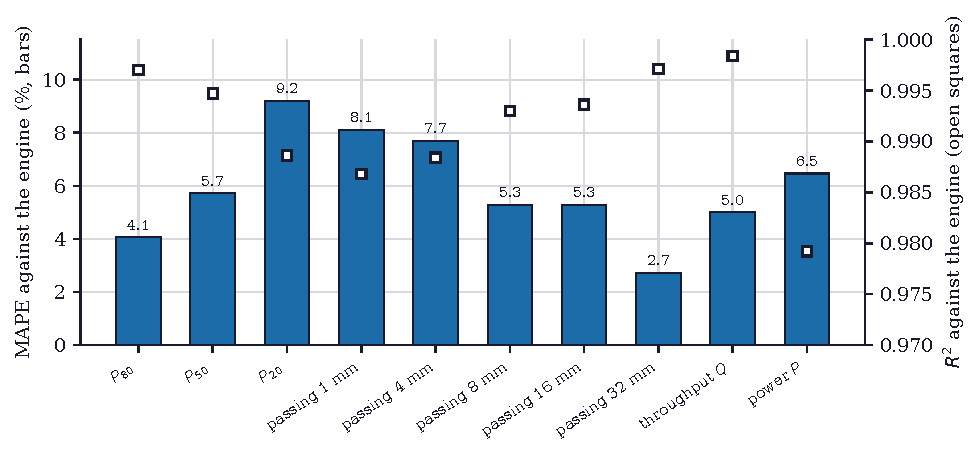
\includegraphics[width=0.85\textwidth]{fig-surrogate.pdf}
\caption{The surrogate against the engine per output on the independent held-out draw of $2196$ points: $R^2$ (bars, left axis) and MAPE in percent
(squares, right axis), computed through onnxruntime on the shipped float32 graph. Read from \texttt{model-metrics.json}.}
\label{fig:surrogate}
\end{figure}

\begin{table}[!t]
\centering
\caption{Surrogate accuracy per output against the engine on the held-out draw: $R^2$ and MAPE of the float32 graph, MAPE of the int8 graph and the difference
in points. Generated from \texttt{model-metrics.json}.}
\label{tab:surrogate}
\footnotesize
% generated by figures/make_tables.py; do not edit by hand
\begin{tabular}{@{}l rrrr@{}}
\toprule
Output & $R^2$ (float32) & MAPE float32 (\%) & MAPE int8 (\%) & Difference (points) \\
\midrule
$P_{80}$ & $0.9970$ & $4.063$ & $4.568$ & $0.505$ \\
$P_{50}$ & $0.9947$ & $5.732$ & $6.125$ & $0.393$ \\
$P_{20}$ & $0.9886$ & $9.213$ & $9.480$ & $0.267$ \\
passing 1 mm & $0.9868$ & $8.115$ & $8.329$ & $0.214$ \\
passing 4 mm & $0.9884$ & $7.700$ & $7.909$ & $0.209$ \\
passing 8 mm & $0.9930$ & $5.296$ & $5.644$ & $0.348$ \\
passing 16 mm & $0.9936$ & $5.293$ & $5.538$ & $0.245$ \\
passing 32 mm & $0.9971$ & $2.730$ & $2.869$ & $0.139$ \\
throughput & $0.9984$ & $5.017$ & $5.434$ & $0.417$ \\
power & $0.9792$ & $6.466$ & $6.431$ & $-0.035$ \\
\bottomrule
\end{tabular}

\end{table}

\begin{table}[!t]
\centering
\caption{The autoencoder's extrapolation score against the envelope check on the same $2196$ held-out points and $2196$ planted off-manifold points:
false-alarm and detection rates, and the threshold and mean training score of the score. Generated from \texttt{model-metrics.json} and \texttt{psd-ae.json}.}
\label{tab:anomaly}
\footnotesize
% generated by figures/make_tables.py; do not edit by hand
\begin{tabular}{@{}l rr@{}}
\toprule
Quantity & Autoencoder & Envelope check \\
\midrule
False-alarm rate on the held-out draw & $0.0100$ & $0.0000$ \\
Detection rate on planted off-manifold points & $0.2796$ & $0.1389$ \\
Points scored (held-out, planted) & $2196$, $2196$ & $2196$, $2196$ \\
Alarm threshold (99th percentile of training scores) & $0.24454$ & -- \\
Mean training reconstruction score & $0.05181$ & -- \\
\bottomrule
\end{tabular}

\end{table}

\subsection{The drift projection}\label{sec:results-drift}

Figure~\ref{fig:drift} gives the drift projection of case S01 for the three targets of the shared reference table. A target $3\%$ above the current
$P_{80}$ ($28.53$~mm) allows the setting to open by $1.04$~mm, a target $10\%$ above ($30.47$~mm) by $3.21$~mm, and a target $30\%$ above ($36.01$~mm) by
$8.67$~mm. The hours to the target are inversely proportional to the drift rate: at $0.1$~mm/h the three openings last $10.4$, $32.1$ and $86.7$~h. The
$45$~h re-set interval of one plant is reached by the $10\%$ target at a drift of $0.071$~mm/h; at a faster drift that target is left before the
re-set. The figure is a what-if on the engine: the product asserts no drift rate, and the reader supplies the one measured at the plant, for example
from the movement of the adjustment ring between two liner changes.

\begin{figure}[!t]
\centering
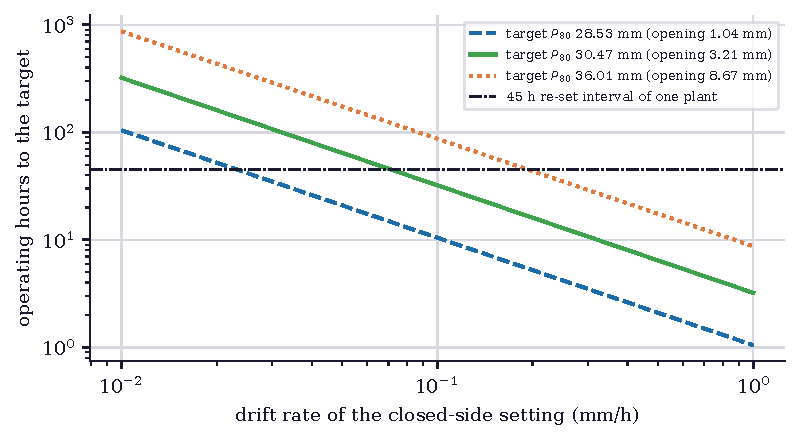
\includegraphics[width=0.72\textwidth]{fig-drift.pdf}
\caption{Operating hours until the product $P_{80}$ of case S01 reaches a target, against the drift rate of the closed-side setting, for targets $3$, $10$ and
$30\%$ above the current $P_{80}$ from the shared reference table, with the $45$~h re-set interval of one plant as reference.}
\label{fig:drift}
\end{figure}
